\documentclass{vgtc}
\graphicspath{{figs/}}
\usepackage{fontspec}
\setmainfont{texgyretermes}[Extension=.otf, UprightFont=*-regular, BoldFont=*-bold, ItalicFont=*-italic, BoldItalicFont=*-bolditalic]
\usepackage{booktabs}
\usepackage{xcolor}
\definecolor{judgered}{HTML}{E60023}
\definecolor{audnavy}{HTML}{0A3069}
\definecolor{promptbg}{HTML}{F3F4F6}

\onlineid{0}
\vgtccategory{Research}
\vgtcinsertpkg

\title{LLM Chart Judges Reward Labels, Not What Audiences Upvote}

\newif\ifanonymous\anonymousfalse
\ifanonymous
  \author{Anonymous Author(s)\\ \scriptsize Affiliation withheld for review}
\else
  \author{Rahul Chaudhary\\ \scriptsize Pinterest, New York, NY, USA}
\fi

\teaser{
  \centering
  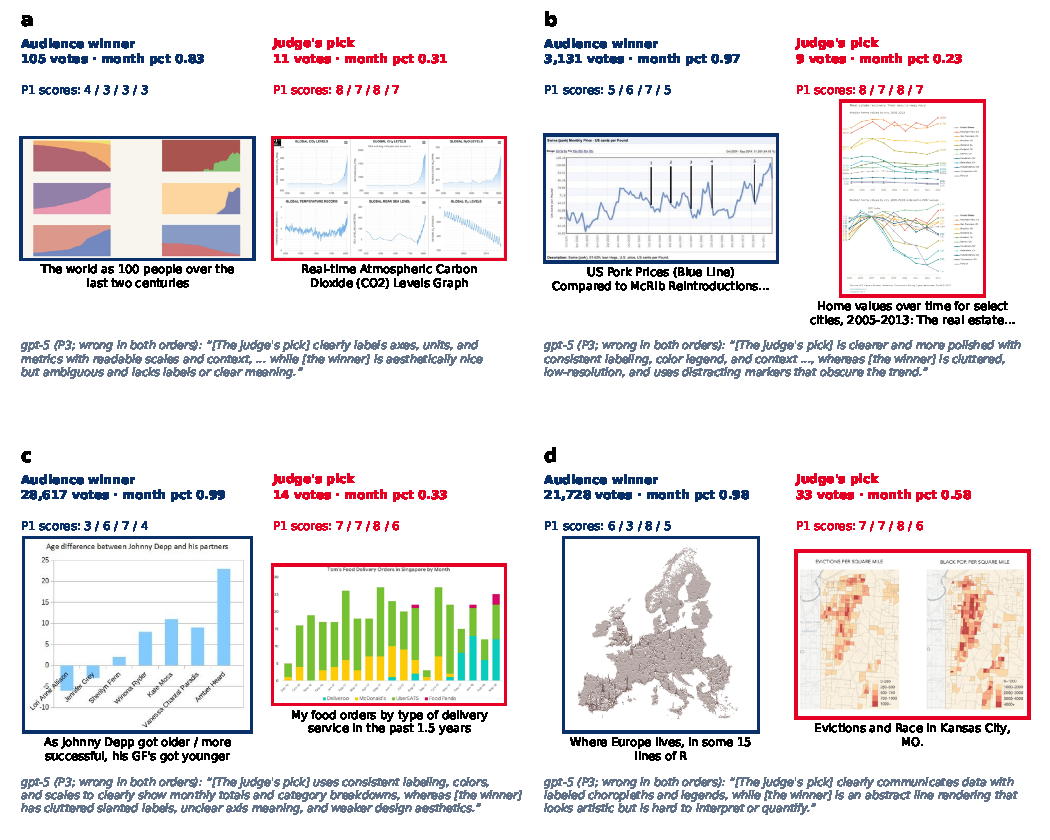
\includegraphics[width=\linewidth, alt={Four pairs of charts from r/dataisbeautiful. In each pair the audience strongly preferred the left chart, but every LLM judge scored the right chart higher, citing labels, legends and clarity.}]{fig5_examples.pdf}
  \refstepcounter{figure}\label{fig:teaser}
  \par\vspace{2pt}{\captionfonts Figure~\thefigure: Four pairs posted in the same week with the same chart type. The audience winner ({\color{audnavy}navy}) received 9--2{,}000$\times$ the votes of the chart the judges preferred ({\color{judgered}red}). P1 scores are listed as gpt-5 / Claude Haiku 4.5 / Gemini 2.5 Flash / Claude Sonnet 5.5. In 15 of the 16 judge--pair cases the judge scores the less-voted chart higher, and the remaining case is a tie. Quotes are gpt-5's reasons from a pairwise prompt that picked the loser in both A/B orders; ``Chart A/B'' is replaced by a bracketed referent. The judges cite labels, legends, and annotation. The audience rewarded a striking idea (a), a joke (b), a celebrity topic (c), and a minimal, artful map (d).\par}
}

\abstract{Multimodal LLMs now score the charts that AI agents generate, and they are validated by agreement with expert ratings. We test whether such judges also agree with what a public audience rewards. From 34{,}556 cleaned r/dataisbeautiful charts (2012--2025) we build 2{,}000 pairs of charts posted in the same week with the same chart type, where one received at least five times the other's votes. An image-blind baseline that reads only the title and posting time picks the winner 59.1\% of the time. In a pre-registered analysis on identical pairs, gpt-5, Claude Haiku 4.5, and Gemini 2.5 Flash pick it 55.5--57.6\% of the time, and the frontier Claude Sonnet 5.5 picks it 57.8\% of the time on 1{,}000 pairs. For every judge we reject an advantage of four points or more over the baseline (one-sided $p\le0.002$), and Haiku is significantly worse. A tie-free AUC comparison ranks every judge below the baseline. The judges do add some independent signal, but none outperforms titles and timing. The same scores correlate 0.44--0.49 with expert ratings and only 0.08--0.13 with audience vote percentile. Every judge rewards text-heavy charts ($+0.31$ to $+0.51$ per SD of OCR word count), while the audience does not ($-0.02$). Agreement with experts does not imply agreement with audiences.}

\keywords{LLM-as-a-judge, visualization quality, audience engagement, equivalence testing, Reddit.}

\begin{document}

\firstsection{Introduction}
\maketitle

Multimodal LLMs increasingly judge charts produced by AI agents: they grade benchmark and challenge entries and act as evaluators in product pipelines. Such a judge is usually validated against experts. VisJudge-Bench~\cite{xie2026visjudge}, for example, reports that GPT-5 correlates 0.428 with expert quality ratings on 3{,}090 visualizations and that a fine-tuned 7B model reaches 0.687.

Many charts are made for a public audience, and no one has tested whether these judges reward what that audience rewards. Audience preference is hard to measure, because raw engagement mostly reflects timing, title, and topic~\cite{kauer2021public}. r/dataisbeautiful offers 13 years of charts with vote counts, packaged as beautiVis~\cite{lin2026beautivis}. We compare each chart only with a close neighbor: a chart posted in the same ISO week, with the same chart type, where one of the two received at least five times the other's votes. We then ask whether a judge picks the audience winner more often than a baseline that never sees the image.

Our contributions are:
\begin{itemize}
\item a controlled pairwise protocol and an image-blind baseline for measuring the audience alignment of chart judges;
\item a pre-registered equivalence analysis showing that four LLM judges, including a frontier model, do not beat titles and timing by four points or more, and one is significantly worse, although the same prompt reaches expert-level agreement;
\item evidence that judges systematically reward text-heavy, labeled charts, a preference the audience does not share.
\end{itemize}

\section{Related Work}
\textbf{LLMs as visualization judges.} VisJudge-Bench~\cite{xie2026visjudge} scores charts on six expert dimensions grouped as fidelity, expressiveness, and aesthetics, and finds moderate agreement between models and experts. Seto et al.~\cite{seto2026literacy} report that frontier models exceed human scores on a visualization-literacy test but struggle to judge whether a chart is misleading without leading prompts. Panda~\cite{panda2026personas} prompts LLMs with literacy-stratified personas and compares them with published human responses. Li et al.~\cite{li2026beauty} compare LLM and human choices of the most pleasing network layout, and Jeon et al.~\cite{jeon2026llmsee} compare how humans and LLMs describe the same charts. All of these use experts, lab participants, or study instruments as the reference. We use the votes of a public audience. Position bias in pairwise LLM judging is well documented for text~\cite{zheng2023judging}; we report it for charts.

\textbf{Audiences on r/dataisbeautiful.} Kauer et al.~\cite{kauer2021public} found that comments on the subreddit mostly discuss topic and insight and rarely discuss design. beautiVis~\cite{lin2026beautivis} provides 52{,}836 visualization posts with GPT-4o chart-type labels mapped to MASSVIS-style categories~\cite{borkin2013memorable}.

\section{Data, Pairs, and Baseline}
\textbf{Cleaning.} From the 52{,}836 beautiVis rows we removed, in order:
\begin{itemize}
\item blank images (148, mostly video thumbnails);
\item posts with an empty or ``Other'' chart type (6{,}449);
\item images whose short side is under 300\,px (1{,}806);
\item posts with fewer than 5 votes (8{,}505), mostly removed or spam posts;
\item near-duplicate images (1{,}372; perceptual-hash distance $\le$2, keeping the earliest post).
\end{itemize}
Groups of three or more near-identical images with unrelated titles are link previews, and we removed them entirely. No rule looks at votes. This leaves 34{,}556 posts, 31{,}542 of them with a single chart type (Supplement S1).

\textbf{Pairs.} We bucket single-type posts by ISO week $\times$ chart type and form \emph{clear} pairs, in which the winner has at least 5 times the loser's votes and at least 50 votes. Each bucket contributes at most three pairs, and each post is used at most once. Pairs are drawn round-robin over years, so every year from 2012 to 2025 appears, and no chart type exceeds 25\%. The display order is randomized. This gives 2{,}000 pairs with a median vote ratio of 32.

\textbf{Image-blind baseline.} An L2-regularized logistic regression predicts the winner from the difference between the two posts' features: title TF-IDF, title length, an \texttt{[OC]} (original content) flag, posting hour, and weekday. Folds are grouped by month, and we use out-of-fold predictions. The baseline picks the winner in 59.1\% of the 2{,}000 pairs (95\% CI 57.0--61.2; AUC 0.623).

\section{Judges and Analysis Plan}
Every judge sees the same standardized JPEG (white background, long side $\le$1536\,px) and never sees the title. The primary prompt, P1, asks for a holistic score:

\smallskip
\noindent\colorbox{promptbg}{\parbox{\dimexpr\columnwidth-2\fboxsep\relax}{\scriptsize\ttfamily You are judging the quality of a data visualization. Rate this chart from 1 (very poor) to 10 (excellent), considering how clearly it communicates its data, how well it is designed, and how visually appealing it is. Respond with JSON only: \{"score": <integer 1-10>, "reason": "<one sentence>"\}}}
\smallskip

\noindent A pair is credited 1 if the audience winner scores higher, 0.5 on a tie, and 0 otherwise.

Three main judges score all 4{,}000 images: gpt-5 (minimal reasoning), Claude Haiku 4.5, and Gemini 2.5 Flash (both at temperature 0). Claude Sonnet 5.5 (low effort) is the frontier judge and scores the first 1{,}000 pairs. Of 14{,}000 P1 requests, one failed to parse and is counted as a tie. As a check of our setup, a rubric prompt gives gpt-5 a Pearson $r$ of 0.414 against expert scores on 150 VisJudge-Bench items, matching the published 0.428 (Supplement S3).

We wrote the analysis plan before running the 2{,}000-pair evaluation (Supplement S5). For each judge, the paired accuracy difference (judge minus baseline) is tested with two one-sided tests (TOST) against a margin of $\pm$4 points at $\alpha=0.05$. A judge is called equivalent when its 90\% bootstrap CI (10{,}000 resamples) lies inside the margin. As a sensitivity check we repeat the analysis on the 1{,}500 pairs that no judge saw during development. Position bias is measured separately with a pairwise prompt run in both A/B orders.

\section{Results}
\begin{table}[tb]
  \caption{P1 results on identical clear pairs. $\Delta$: judge minus baseline accuracy in points, with its 90\% bootstrap CI. $p_{>+4}$: one-sided test that the judge beats the baseline by 4 points or more. AUC: ranking quality of the judge's score difference alone, which needs no tie rule. LR $p$: likelihood-ratio test of adding the judge's score difference to the baseline model. $^\dagger$Sonnet is compared on the first 1{,}000 pairs, where the baseline scores 59.6\% (AUC 0.630).}
  \label{tab:main}
  \scriptsize
  \centering
  \setlength{\tabcolsep}{2.6pt}
  \resizebox{\columnwidth}{!}{%
  \begin{tabular}{@{}lrcrccc@{}}
  \toprule
  Judge (P1) & $n$ & Accuracy (95\% CI) & $\Delta$ [90\% CI] & $p_{>+4}$ & AUC & LR $p$ \\
  \midrule
  Image-blind baseline & 2{,}000 & .591 (.570--.612) & -- & -- & .623 & -- \\
  gpt-5 & 2{,}000 & .564 (.544--.583) & $-2.8$ [$-5.1$, $-0.3$] & $2\!\times\!10^{-6}$ & .581 & $<10^{-4}$ \\
  Claude Haiku 4.5 & 2{,}000 & .555 (.537--.572) & $-3.7$ [$-5.9$, $-1.3$] & $3\!\times\!10^{-8}$ & .571 & $<10^{-4}$ \\
  Gemini 2.5 Flash & 2{,}000 & .576 (.558--.593) & $-1.5$ [$-3.9$, $+0.9$] & $4\!\times\!10^{-5}$ & .603 & $<10^{-4}$ \\
  Claude Sonnet 5.5$^\dagger$ & 1{,}000 & .578 (.551--.604) & $-1.9$ [$-5.2$, $+1.5$] & .002 & .604 & -- \\
  \bottomrule
  \end{tabular}}
\end{table}

\begin{figure}[tb]
  \centering
  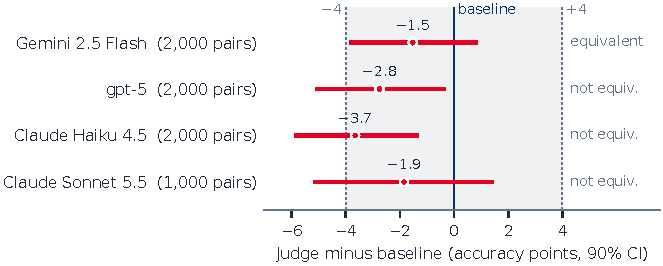
\includegraphics[width=\columnwidth, alt={Forest plot of judge-minus-baseline accuracy with 90 percent confidence intervals inside a shaded band from minus four to plus four points. All four point estimates are below zero, and every interval ends at or below plus 1.5 points.}]{fig7_tost.pdf}
  \caption{Pre-registered equivalence test. Each {\color{judgered}red} interval is a judge's accuracy minus the image-blind baseline ({\color{audnavy}navy} line), with its 90\% CI. The shaded band is the $\pm$4-point margin. Every point estimate is below the baseline, and no upper bound exceeds $+1.5$ points.}
  \label{fig:tost}
\end{figure}

\textbf{RQ1: No judge beats titles and timing.} No judge beats the image-blind baseline by 4 points or more (\cref{tab:main}, \cref{fig:tost}). Every point estimate is below the baseline, and the upper 90\% bounds range from $-1.3$ to $+1.5$ points. For every judge we reject an advantage of four points or more ($p\le0.002$). Under the pre-registered two-sided rule, Gemini Flash is equivalent to the baseline (TOST $p=0.039$). gpt-5 and Haiku are not equivalent only because they may be more than four points \emph{worse}, and Haiku is significantly worse (95\% CI $[-6.4, -0.9]$). The frontier judge does not close the gap: on its 1{,}000 pairs Sonnet 5.5 is equivalent to gpt-5 ($+0.7$ points, TOST $p=0.004$) and to Flash ($+0.5$, $p=0.002$). On the 1{,}500 pairs unseen during development the differences barely move ($-2.8$, $-3.2$, and $-1.4$ points).

\textbf{Ties.} A 1--10 scale ties on 23--35\% of pairs, and a tie earns 0.5, which pulls a judge toward chance. Two post-hoc checks remove ties. First, on the pairs where a judge gives different scores, its accuracy (58.1--61.7\%) differs from the baseline on the same pairs by $-1.6$ to $+3.3$ points, and no difference is significant. Gemini Flash, which ties most often, comes closest ($+3.3$, 95\% CI $[-0.3, +7.1]$), so the four-point bound holds under our pre-registered scoring but not on Flash's decisive pairs alone. Second, ranked by AUC, every judge falls below the baseline (0.571--0.604 against 0.623--0.630), significantly so for gpt-5 ($-0.042$, 95\% CI $[-0.075, -0.007]$) and Haiku ($-0.052$, $[-0.086, -0.019]$).

The judges are not uninformative. Adding a judge's score difference to the baseline's out-of-fold logit improves the fit for every judge (likelihood-ratio $\chi^2$ of 17--40, $p<10^{-4}$), but AUC rises only from 0.623 to 0.634--0.649. The judges see something that titles and timing miss, yet on their own they predict votes less well than titles and timing do.

\textbf{Expert alignment does not transfer.} Both comparisons use the same P1 scores and the same rank correlation (Spearman $\rho$). On 150 VisJudge-Bench items, judge scores correlate $\rho=0.44$--0.49 with expert ratings. On the 4{,}000 audience images, they correlate only $\rho=0.08$--0.13 with each post's vote percentile within its month (Sonnet: 0.12 on 2{,}000 images).

\begin{figure}[tb]
  \centering
  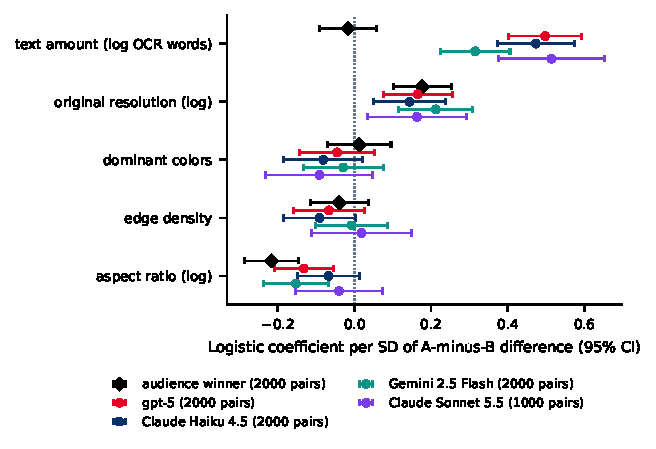
\includegraphics[width=\columnwidth, alt={Dot plot of logistic coefficients for five image features. For text amount the audience coefficient is near zero while all four judges are between 0.3 and 0.5. For the other four features the audience and judge intervals overlap or lie close together.}]{fig8_bias_all.pdf}
  \caption{Image features that predict the audience winner ({\color{audnavy}navy}) and each judge's P1 pick ({\color{judgered}red}), as logistic coefficients on the A-minus-B feature difference (Sonnet on 1{,}000 pairs, others on 2{,}000). Text amount (shaded) is where judges and audience diverge most.}
  \label{fig:bias}
\end{figure}

\textbf{RQ2: Judges reward text; the audience does not.} We computed five features per image (OCR word count, dominant-color count, edge density, aspect ratio, and original resolution) and fit logistic regressions on the A-minus-B feature differences, separately for the audience winner and for each judge's pick (\cref{fig:bias}). On resolution, color count, and edge density, judges and audience agree. Text is the clear exception: every judge favors the chart with more words ($+0.31$ to $+0.51$ per SD, SE 0.05--0.07), while the audience coefficient is $-0.02$ (SE 0.04). The judges' stated reasons match this pattern (\cref{fig:teaser}). They praise ``consistent labeling,'' ``color legend,'' and ``readable scales,'' and they penalize charts that are ``abstract'' or ``ambiguous.'' The audience winners in \cref{fig:teaser} are a striking idea, a joke, a celebrity topic, and a minimalist map without a single label.

\textbf{RQ3: Position bias.} With a pairwise prompt (``Which one is the better visualization overall?'') run in both orders, gpt-5 and Haiku change their answer on 18\% of 250 pairs. Gemini Flash changes its answer on 53\% of 500 pairs and picks whichever chart is shown first 77\% of the time, so its single-order pairwise choices are close to arbitrary. Pairwise accuracy is no higher than P1 accuracy for any judge (Supplement S2).

\section{Discussion}
The judges reproduce published expert-alignment numbers, yet none predicts audience votes better than a model that reads only titles and timestamps. The disagreement has a direction. The judges apply a checklist of labeling and annotation, and many charts the audience rewards would fail that checklist. For anyone who scores chart-generating agents, an LLM judge's score measures conformance to conventions, not engagement. Systems that aim to engage an audience need audience data or an audience-calibrated judge, and pairwise judging should always be run in both orders.

\section{Limitations}
\begin{itemize}
\item \textbf{One noisy audience.} Votes are noisy, and r/dataisbeautiful is one community whose rules shape what gets posted.
\item \textbf{Lopsided pairs.} Clear pairs are very unequal, and some losers may be low-effort posts. Such losers should be easy to spot, which favors the judges, not the baseline.
\item \textbf{Quality prompts.} We test judges as they are used, with prompts about quality. We did not test whether a prompt that asks which chart got more votes does better.
\item \textbf{Indirect evidence for topics.} Our suggestion that audiences respond to topic rests on the strength of the title baseline and on prior work~\cite{kauer2021public}; we did not code topics directly.
\item \textbf{Models and labels.} Budget kept Sonnet 5.5 to 1{,}000 pairs. We did not test an expert-tuned judge (VisJudge-7B), and chart types are beautiVis's GPT-4o labels.
\end{itemize}

\section*{Supplemental Materials}
\label{sec:supplemental_materials}
The supplement contains S1, cleaning details and deviations from our original plan; S2, the rubric (P2) and pairwise (P3) prompts, a title-only control, and close pairs; S3, calibration on VisJudge-Bench; S4, memorization checks; and S5, the pre-registration. \ifanonymous Code, prompts, post identifiers and permalinks, all raw judge responses with token usage, and all analysis tables are in an anonymized repository (link withheld for review).\else Code, prompts, post identifiers and permalinks, all raw judge responses with token usage, and all analysis tables are at \url{https://github.com/vibedatascience/chart-judges-vs-audience}.\fi{} Images are not redistributed.\ifanonymous\else{} This work was done in a personal capacity; the views expressed are the author's own and do not represent Pinterest.\fi

\section*{Figure Credits}
\label{sec:figure_credits}
\Cref{fig:teaser} reproduces eight charts posted to r/dataisbeautiful, retrieved through beautiVis~\cite{lin2026beautivis}, and shown here for commentary. Credits, as Reddit user and post ID: (a) u/RightFloor \texttt{5jk2ub}, u/Sourcecode12 \texttt{5jn2mu}; (b) u/OMGLMAOWTF\_com \texttt{2ionwm}, u/marriedacarrot \texttt{2it1p7}; (c) u/Smart\_Ass\_Pawn \texttt{8awx8s}, u/tomeczak \texttt{8awz4p}; (d) u/halhen \texttt{671s4d}, u/AbeDrinkin \texttt{66ifjl}. Each post is at \texttt{reddit.com/r/dataisbeautiful/comments/<id>}.

\bibliographystyle{abbrv-doi}
\bibliography{refs}
\end{document}
